\documentclass{article}
\usepackage{graphicx} % Required for inserting images
\usepackage[margin=3cm]{geometry}
\usepackage{biblatex}
\usepackage{hyperref}
\usepackage{cleveref}
\usepackage{listings}
\usepackage{tabularx}


\hypersetup{
    colorlinks=true,
    linkcolor=blue,
    filecolor=magenta,      
    urlcolor=cyan,
    pdftitle={Overleaf Example},
    pdfpagemode=FullScreen,
    }

\title{NEA \\Route Card and Route Planning tool}
\author{Jonty Beglin}
\date{April 2024}

\newcommand{\Q}{\bigskip\bfseries Q: }
\newcommand{\A}{\par\textbf{A:} \normalfont}

\newcommand{\Adv}{\bigskip\textbf{Advantages: }}
\newcommand{\Dis}{\bigskip\textbf{Disadvantages: }}

\newcommand{\testtable}[6]{
    \begin{center}
        \textbf{#1}
        \vspace{0.125cm}
        \vspace{0.25cm}
        \begin{tabularx}{\textwidth}{ |X|X|X|X| }
            \hline
            Testing & Objective & Pass/Fail & Notes \\
            \hline
            #2 & #3 & #4 & #5 \\
            \hline
        \end{tabularx}
        \\
        \vspace{0.25cm}
        \url{#6}
    \end{center}
}

\begin{document}

\maketitle

\newpage

\tableofcontents

\newpage


\section{Analysis}

    \subsection{The Problem}

        I would like to create a tool that allows users to plan hiking routes on an interactive UI featuring a map and waypoint capabilities. The tool should then be able to return to the user a route card that the user can use while on their hike to navigate along the path they have created within the program with useful information they may want such as bearings, walking times, distances and place names. An example of what could be displayed in the program can be seen in \cref{fig:example_map_dartmoor}.

        \begin{figure}[h]
            \centering
            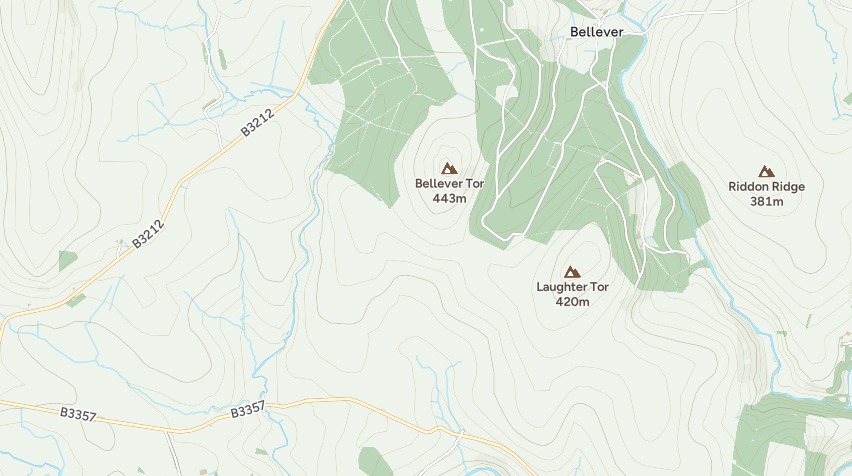
\includegraphics[width=0.75\textwidth]{Photos/Example/OSmapsExampleDartmoor.png}
            \caption{Example of a map which could be displayed within the program}
            \label{fig:example_map_dartmoor}
         \end{figure}

         Currently many people I know use pen and paper with physical maps to measure out distance and do manual calculations to create their route cards. I believe many people would benefit from this as it should be faster, easier and more accurate than traditional methods. I would further like to add options to load and save routes meaning users can edit their previously created routes.
         
         I would like to implement a feature to snap to paths to get more accurate readings of the path distance and time taken to walk a path. However, depending on which APIs are used and what data is available this may not be possible to achieve in some circumstances due to the disparity between the real world and the data online.
         
        \begin{figure}[h]
            \centering
            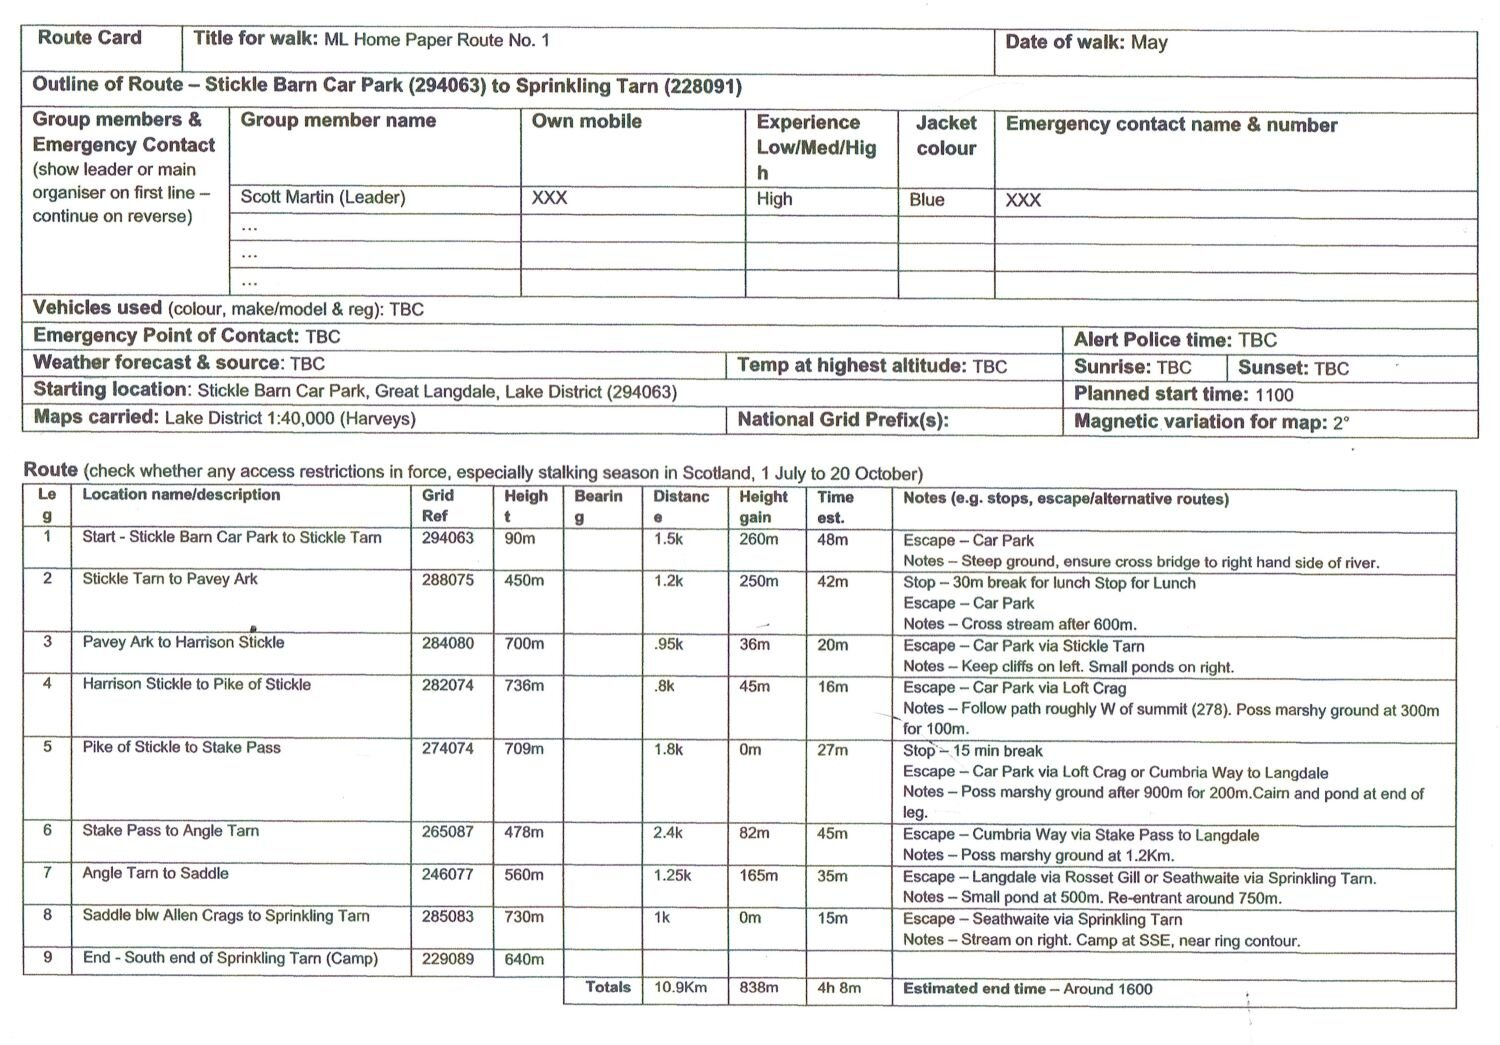
\includegraphics[width=0.75\textwidth]{Photos/Example/RouteCardExample.jpg}
            \caption{Example of a Route Card which could be generated from the program}
            \label{fig:example_route_card}
         \end{figure}
         
         I think there should be options for how the route card will be laid out, potentially allowing the user to directly edit the route card which will be outputted. This may be a sub-program within the main program which enables the user to view and edit the data of the route card. An example route card which the program should aim to output can be seen in \cref{fig:example_route_card}.

    \subsection{Mapping APIs}

        Choosing the most suitable API for gathering map data is paramount to the project's success. The map data needs to be able to be accessed relatively quickly and reliably, potentially the user could potentially interact with an interactive map as seen in Google Maps and draw the route in real-time, however, this may be out of the scope of the project, so instead I could allow the user to use an interactive map to find a snapshot location of their "work area" where then they can draw their route on top of which will have an inbuilt scale automatically scaled to the same scale as when they were using the interactive map. The user's waypoint locations could be saved to allow for the later creation of a route card or as previously mentioned create a route which can be edited or expanded upon later. Optimally the mapping API should allow me to feed in some latitude and longitude and it feed back some mapping data in the form of a photo or other source which can then be overlaid onto the screen and I could use some module such as pygame or tkinter in python to move based on the user's actions.
    
\newpage

\section{Documented Design}

    

\newpage
    
\section{Technical Solution}

    

\newpage

\section{Testing}

    

\newpage

\section{Evaluation}

    
    
\end{document}
